\section{Introduction}\label{introduction}

\begin{frame}{Basic Analyses}

\center
\textbf{Basic Analyses}: The analyses taught in the first stats course
\vspace{12pt}

\columnsbegin

\begin{column}{0.48\textwidth}
   These include:
   \begin{enumerate}
   \item T-tests
   \item ANOVA
   \item Linear Regression
   \end{enumerate}
   These allow us to assess relationships like that in the figure.
\end{column}\begin{column}{0.48\textwidth}
    \begin{center}
     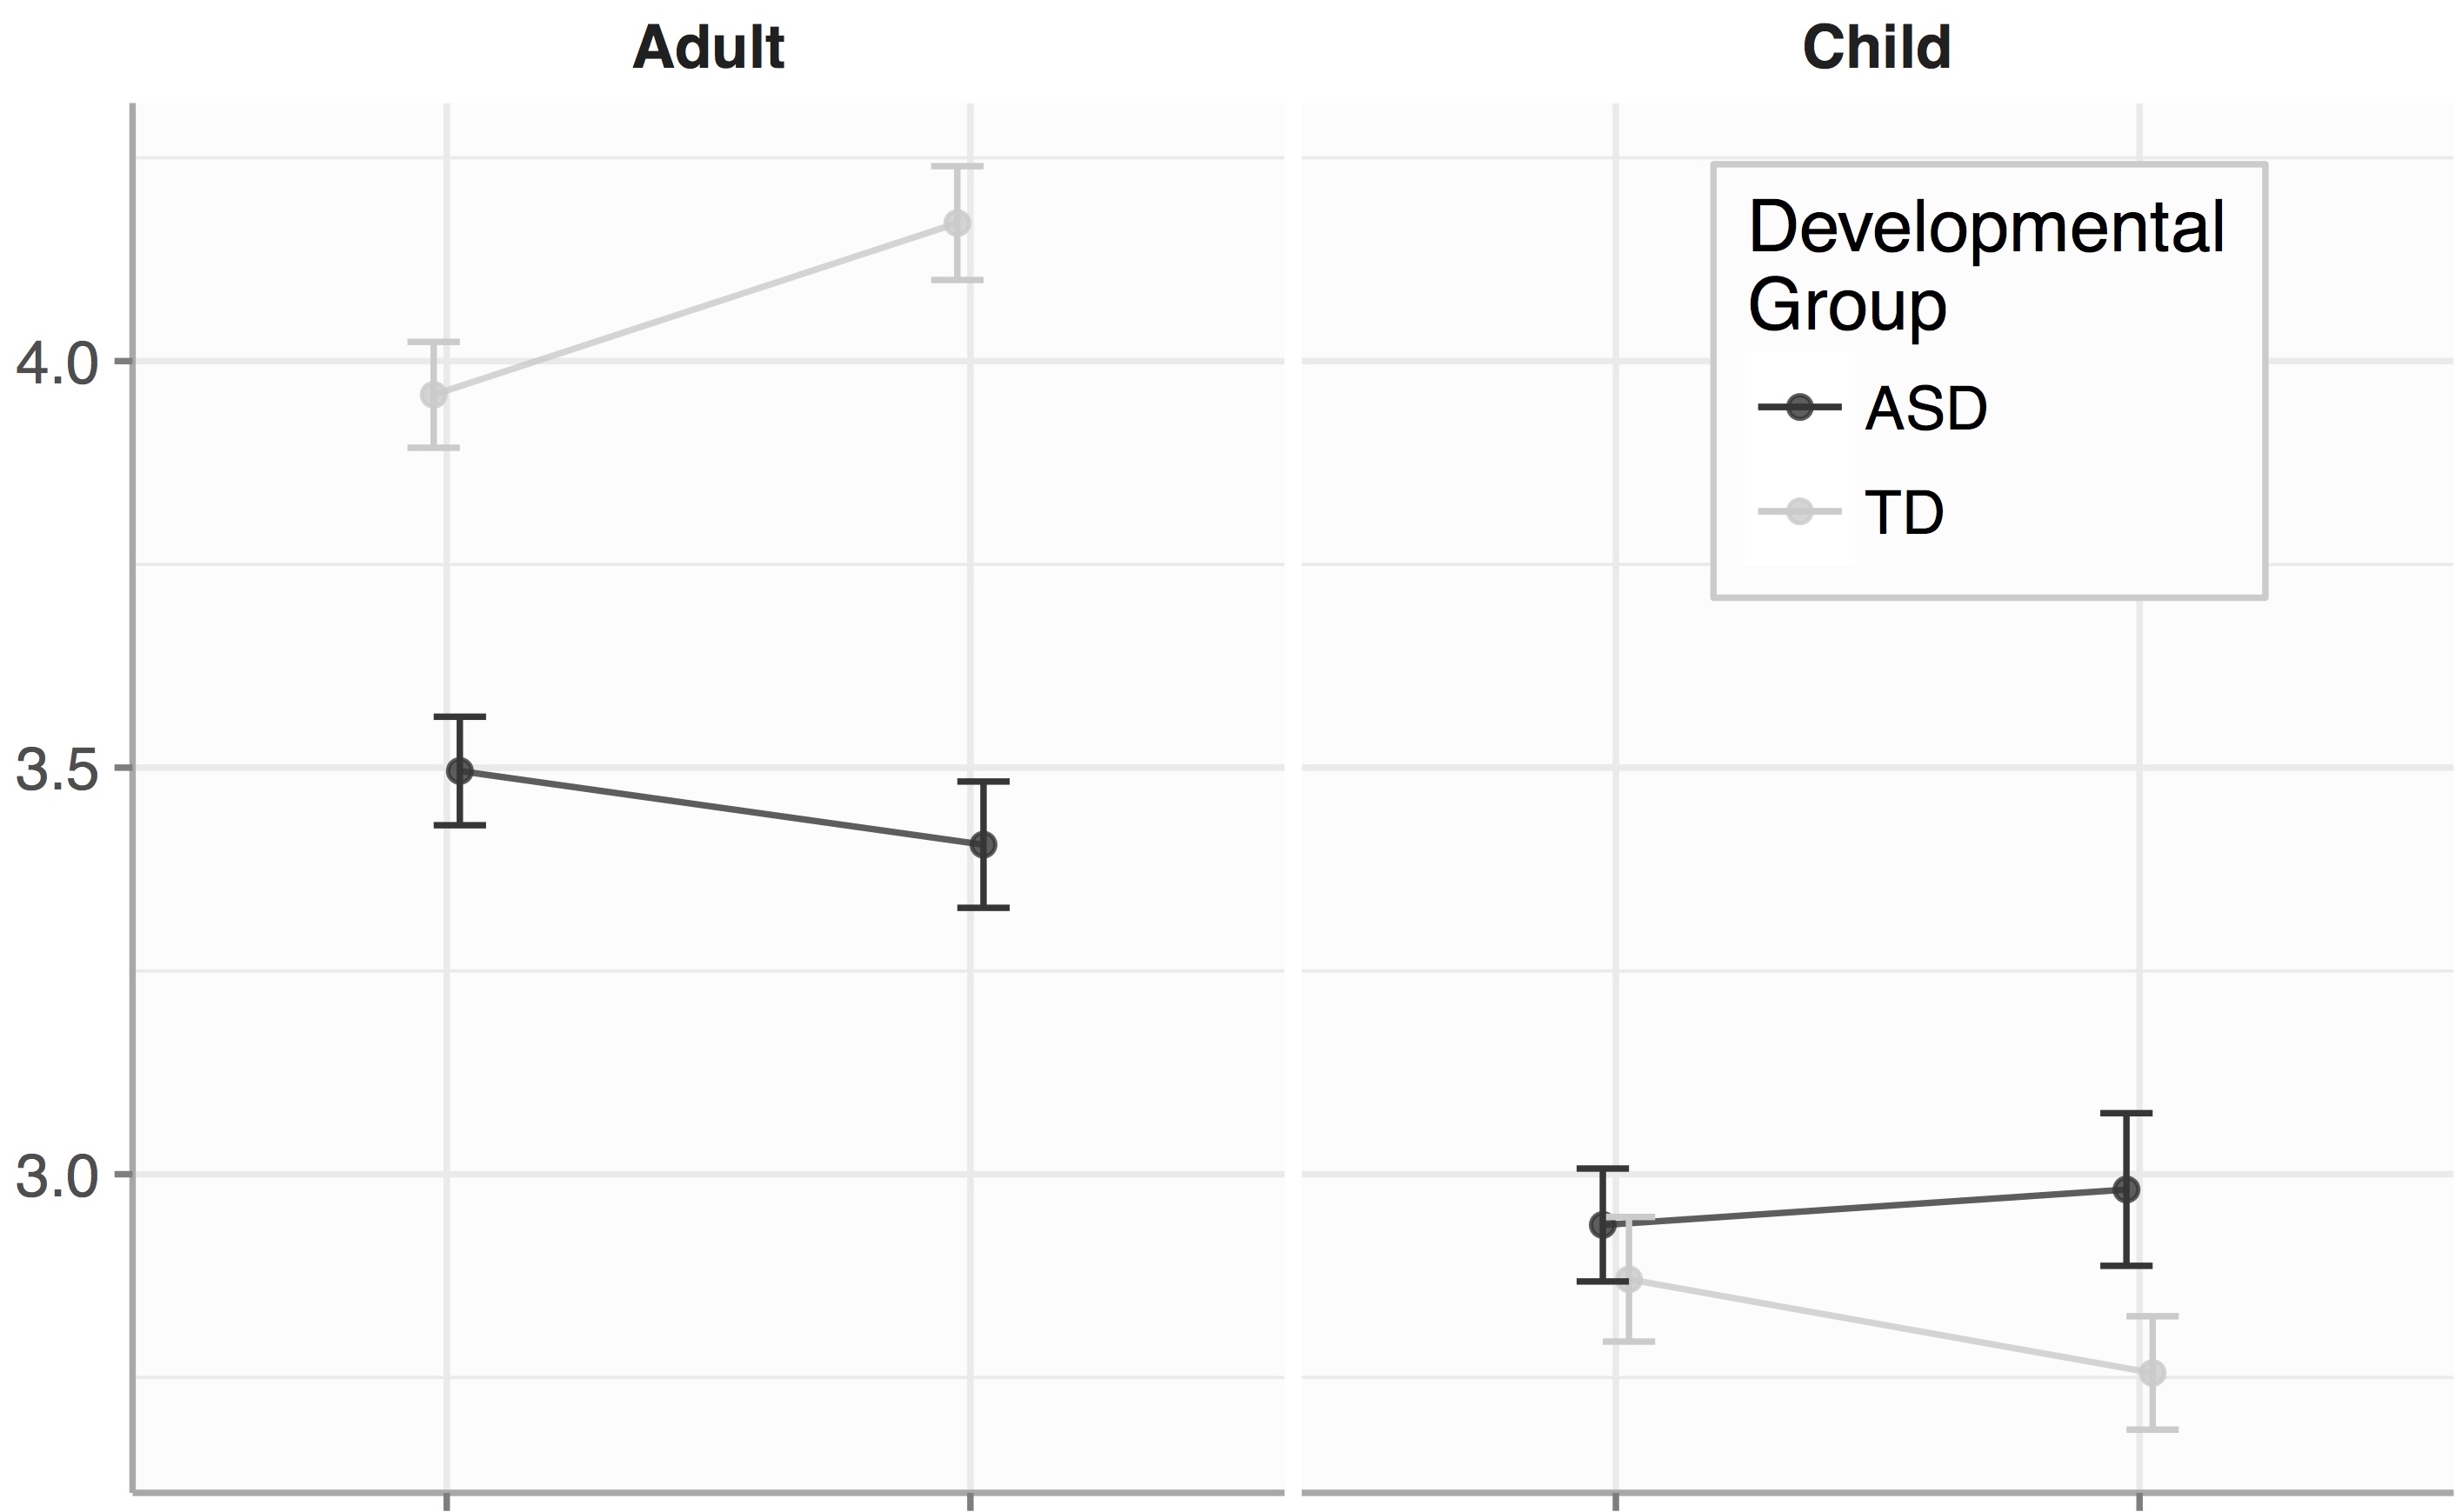
\includegraphics[width=\textwidth]{Figures/FigureInteraction.jpg}
     \end{center}
\end{column}

\columnsend

\vspace{12pt} Maybe surprising:\textbackslash{} These all are doing
essentially the same thing!

First, \textbf{T-TESTS!}

\end{frame}

\section{T-tests}\label{t-tests}

\begin{frame}{Three Types}

\Huge

\begin{enumerate}
\item Simple
\item Independent Samples
\item Paired Samples
\end{enumerate}

\end{frame}

\begin{frame}[fragile]{Three Types}

\Large
Each will be demonstrated using:

\normalsize

\begin{Shaded}
\begin{Highlighting}[]
\NormalTok{df <-}\StringTok{ }\KeywordTok{data.frame}\NormalTok{(}\StringTok{"A"}\NormalTok{=}\KeywordTok{sample}\NormalTok{(}\KeywordTok{c}\NormalTok{(}\DecValTok{0}\NormalTok{,}\DecValTok{1}\NormalTok{), }\DecValTok{100}\NormalTok{, }\DataTypeTok{replace =} \OtherTok{TRUE}\NormalTok{),}
                 \StringTok{"B"}\NormalTok{=}\KeywordTok{rnorm}\NormalTok{(}\DecValTok{100}\NormalTok{),}
                 \StringTok{"C"}\NormalTok{=}\KeywordTok{rnorm}\NormalTok{(}\DecValTok{100}\NormalTok{))}
\NormalTok{df}
\end{Highlighting}
\end{Shaded}

\begin{verbatim}
    A           B            C
1   0 -0.49302332 -1.929185797
2   0 -0.74567281 -0.501050403
3   0  0.76942036  0.972653402
4   0  0.26824581  0.325231701
5   1  0.22727798 -0.380874790
6   1 -1.30398561  0.874102358
7   0 -0.56605613  1.977208866
8   0 -1.12392072  0.146750347
9   1 -0.45675323 -0.334580377
10  0 -0.40172414  0.544634441
11  1 -0.93475101 -1.797942295
12  0  0.04203159 -0.132622155
13  1 -0.18467893 -0.893717318
14  1 -0.33613628  0.061449397
15  1  0.02941359 -0.480628073
16  1 -1.78610886 -1.696705424
17  0 -0.71122071  0.454180294
18  0  0.02849750 -1.201685459
19  1 -0.13736917  1.038278899
20  1 -1.77769446  3.996691087
21  1  2.50736115 -0.040838143
22  1 -1.32708108  2.397226520
23  1  0.46250563 -0.445476147
24  0  0.01820506 -0.134544120
25  0 -0.53149927 -0.108403405
26  0 -0.49857211  0.531502743
27  0 -0.12931627  1.045776914
28  0  0.29959365 -0.609399628
29  0  0.70868023  0.893310355
30  0 -2.34465712  0.466828659
31  1  2.35461428 -1.007039151
32  0  0.18516693 -0.630011152
33  1  0.38109574  0.086146930
34  0 -1.50037594  0.769931029
35  1  1.01294134  0.462058165
36  0  0.17617688  1.037405312
37  1 -0.23587310  1.402482400
38  0 -1.20536119  1.544293390
39  0  0.63670426 -1.676491724
40  0  0.44894683  1.098549517
41  1  1.46649678 -0.030864350
42  0  0.31610926 -1.284847001
43  0  0.12732902  0.092517793
44  0 -1.37511387  0.403282393
45  1  0.22185552  0.239633333
46  1 -0.97232711 -1.562281821
47  0  1.07579054  0.295312181
48  1  1.67319829  0.936532869
49  1 -0.13587098  0.141149310
50  1  0.28756610  0.091949510
51  1  0.19555493  0.409750181
52  1  0.27946530 -1.216865564
53  1  0.22727981  1.271984702
54  1 -0.59349020  0.179870318
55  0 -0.28631546 -0.008607799
56  0 -0.27744286 -0.131508169
57  0 -0.25025722  1.189048779
58  1  0.49864026 -0.330117543
59  0 -0.25023787  1.404454445
60  0 -0.92005682 -0.805836558
61  0  0.88076558 -1.549905803
62  0 -1.18825586 -0.666934089
63  1  0.04922399 -0.596816665
64  0 -0.11830691 -0.699348063
65  1 -2.04923164 -0.061401056
66  0 -1.58491253  0.544065160
67  1 -0.76521118  0.651592316
68  0 -0.77052905 -0.194041745
69  1 -1.21897672  2.485709388
70  1  0.07827895  0.683474807
71  0  0.13423961 -0.780690090
72  0  1.11437221 -0.524593928
73  0  0.91489171 -0.364885363
74  0 -0.07964019  1.830271957
75  1 -0.04583834  0.908062819
76  1 -0.74328061  1.774913302
77  0  1.32141135 -0.668074758
78  1 -0.99022267 -0.764126728
79  1  1.46493498  0.166734910
80  0  0.11663702  1.762028794
81  0  0.64543170  0.060136057
82  0 -1.25322755  0.606853182
83  0  0.50980944 -1.015951693
84  1 -0.59070166  1.807842864
85  0 -3.06373843  1.264642852
86  0  2.07723232  0.246492920
87  0 -0.26250516 -0.736596989
88  1  0.47291557  0.166971165
89  0 -0.11191884 -0.735371453
90  1  0.03192378 -0.357579334
91  0 -1.35365044 -0.397938613
92  0 -0.98802199 -0.908032942
93  1  1.46332380 -0.086115014
94  1 -0.50653374 -0.182045115
95  0 -0.34161719  0.273961166
96  0  1.07173985  0.621019150
97  1  0.40251912 -0.747195768
98  0 -0.64835377  0.720099137
99  0  0.37624125  0.198332343
100 1  0.52104226  0.210062004
\end{verbatim}

\end{frame}

\begin{frame}[fragile]{Simple}

\center
Comparing a mean of a variable with \(\mu\).

\begin{Shaded}
\begin{Highlighting}[]
\KeywordTok{t.test}\NormalTok{(df}\OperatorTok{$}\NormalTok{B, }\DataTypeTok{mu =} \DecValTok{0}\NormalTok{)}
\end{Highlighting}
\end{Shaded}

\begin{verbatim}

    One Sample t-test

data:  df$B
t = -1.2338, df = 99, p-value = 0.2202
alternative hypothesis: true mean is not equal to 0
95 percent confidence interval:
 -0.3102355  0.0723451
sample estimates:
 mean of x 
-0.1189452 
\end{verbatim}

\end{frame}

\begin{frame}[fragile]{Independent Samples}

\center
Comparing the means of two groups (\texttt{dfA} is the grouping
variable).

\begin{Shaded}
\begin{Highlighting}[]
\KeywordTok{t.test}\NormalTok{(df}\OperatorTok{$}\NormalTok{B }\OperatorTok{~}\StringTok{ }\NormalTok{df}\OperatorTok{$}\NormalTok{A)}
\end{Highlighting}
\end{Shaded}

\begin{verbatim}

    Welch Two Sample t-test

data:  df$B by df$A
t = -0.91829, df = 87.734, p-value = 0.361
alternative hypothesis: true difference in means is not equal to 0
95 percent confidence interval:
 -0.5715761  0.2103016
sample estimates:
mean in group 0 mean in group 1 
    -0.19842557     -0.01778835 
\end{verbatim}

\end{frame}

\begin{frame}[fragile]{Paired Samples}

\center
Comparing repeated measures (e.g., Pretest vs.~Posttest).

\begin{Shaded}
\begin{Highlighting}[]
\KeywordTok{t.test}\NormalTok{(df}\OperatorTok{$}\NormalTok{B, df}\OperatorTok{$}\NormalTok{C, }\DataTypeTok{paired =} \OtherTok{TRUE}\NormalTok{)}
\end{Highlighting}
\end{Shaded}

\begin{verbatim}

    Paired t-test

data:  df$B and df$C
t = -1.7104, df = 99, p-value = 0.09033
alternative hypothesis: true difference in means is not equal to 0
95 percent confidence interval:
 -0.56702904  0.04202515
sample estimates:
mean of the differences 
             -0.2625019 
\end{verbatim}

\end{frame}

\begin{frame}[fragile]{Testing Assumptions of T-Tests}

T-tests require that the data be normally distributed with approximately
the same variance.

\begin{Shaded}
\begin{Highlighting}[]
\NormalTok{## Normality}
\KeywordTok{par}\NormalTok{(}\DataTypeTok{mfrow =} \KeywordTok{c}\NormalTok{(}\DecValTok{1}\NormalTok{,}\DecValTok{2}\NormalTok{))}
\KeywordTok{hist}\NormalTok{(df}\OperatorTok{$}\NormalTok{B)}
\KeywordTok{qqnorm}\NormalTok{(df}\OperatorTok{$}\NormalTok{B)}
\KeywordTok{abline}\NormalTok{(}\DataTypeTok{a=}\DecValTok{0}\NormalTok{, }\DataTypeTok{b=}\DecValTok{1}\NormalTok{)}
\end{Highlighting}
\end{Shaded}

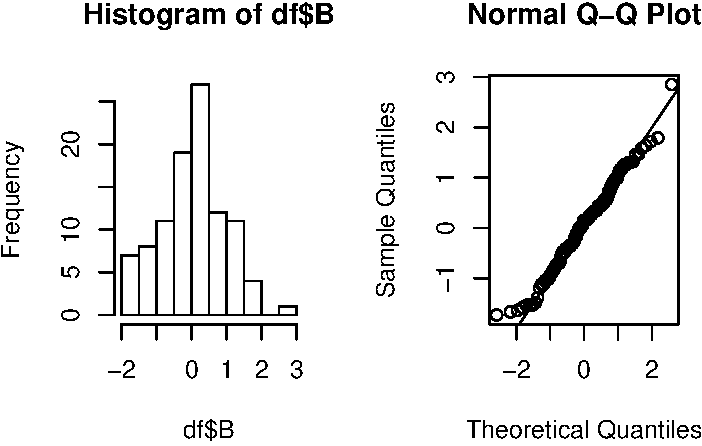
\includegraphics{04_BasicAnalyses_files/figure-beamer/unnamed-chunk-5-1.pdf}

\begin{Shaded}
\begin{Highlighting}[]
\NormalTok{## Variance}
\KeywordTok{var}\NormalTok{(df}\OperatorTok{$}\NormalTok{B)}
\end{Highlighting}
\end{Shaded}

\begin{verbatim}
[1] 0.9294105
\end{verbatim}

\begin{Shaded}
\begin{Highlighting}[]
\KeywordTok{var}\NormalTok{(df}\OperatorTok{$}\NormalTok{C)}
\end{Highlighting}
\end{Shaded}

\begin{verbatim}
[1] 1.021044
\end{verbatim}

\end{frame}

\section{ANOVA}\label{anova}

\begin{frame}[fragile]{Analysis of Variance}

The Analysis of Variance (ANOVA) is highly related to t-tests but can
handle 2+ groups.

\begin{enumerate}
\def\labelenumi{\arabic{enumi}.}
\tightlist
\item
  Provides the same p-value as t-tests
\item
  \(t^2\) = \(F\)
\end{enumerate}

For example:

\begin{Shaded}
\begin{Highlighting}[]
\NormalTok{fit_ano =}\StringTok{ }\KeywordTok{aov}\NormalTok{(df}\OperatorTok{$}\NormalTok{B }\OperatorTok{~}\StringTok{ }\NormalTok{df}\OperatorTok{$}\NormalTok{A)}
\KeywordTok{summary}\NormalTok{(fit_ano)}
\end{Highlighting}
\end{Shaded}

\begin{verbatim}
            Df Sum Sq Mean Sq F value Pr(>F)
df$A         1   0.80  0.8040   0.864  0.355
Residuals   98  91.21  0.9307               
\end{verbatim}

\begin{Shaded}
\begin{Highlighting}[]
\KeywordTok{t.test}\NormalTok{(df}\OperatorTok{$}\NormalTok{B }\OperatorTok{~}\StringTok{ }\NormalTok{df}\OperatorTok{$}\NormalTok{A)}\OperatorTok{$}\NormalTok{p.value}
\end{Highlighting}
\end{Shaded}

\begin{verbatim}
[1] 0.3609868
\end{verbatim}

\end{frame}

\begin{frame}[fragile]{Analysis of Variance}

\begin{Shaded}
\begin{Highlighting}[]
\NormalTok{fit_ano =}\StringTok{ }\KeywordTok{aov}\NormalTok{(df}\OperatorTok{$}\NormalTok{B }\OperatorTok{~}\StringTok{ }\NormalTok{df}\OperatorTok{$}\NormalTok{A)}
\KeywordTok{summary}\NormalTok{(fit_ano)}
\KeywordTok{t.test}\NormalTok{(df}\OperatorTok{$}\NormalTok{B }\OperatorTok{~}\StringTok{ }\NormalTok{df}\OperatorTok{$}\NormalTok{A)}\OperatorTok{$}\NormalTok{p.value}
\end{Highlighting}
\end{Shaded}

Notice in the code:

\begin{itemize}
\tightlist
\item
  We assigned the \texttt{aov()} the name \texttt{fit\_ano} (which we
  could have called anything)
\item
  We used the \texttt{summary()} function to see the F and p values.
\item
  We pulled the p-value right out of the \texttt{t.test()} function.
\end{itemize}

\end{frame}

\begin{frame}{Types}

\huge

\begin{enumerate}
\item One-Way
\item Two-Way (Factorial)
\item Repeated Measures
\item A combination of Factorial and Repeated Measures
\end{enumerate}

\end{frame}

\begin{frame}[fragile]{Types}

We will use the following data set for the examples:

\begin{Shaded}
\begin{Highlighting}[]
\KeywordTok{library}\NormalTok{(tidyverse)}
\NormalTok{df <-}\StringTok{ }\KeywordTok{data.frame}\NormalTok{(}\StringTok{"A"}\NormalTok{=}\KeywordTok{sample}\NormalTok{(}\KeywordTok{c}\NormalTok{(}\DecValTok{0}\NormalTok{,}\DecValTok{1}\NormalTok{), }\DecValTok{100}\NormalTok{, }\DataTypeTok{replace =} \OtherTok{TRUE}\NormalTok{) }\OperatorTok\StringTok{ }\NormalTok{factor,}
                 \StringTok{"B"}\NormalTok{=}\KeywordTok{rnorm}\NormalTok{(}\DecValTok{100}\NormalTok{),}
                 \StringTok{"C"}\NormalTok{=}\KeywordTok{rnorm}\NormalTok{(}\DecValTok{100}\NormalTok{),}
                 \StringTok{"D"}\NormalTok{=}\KeywordTok{sample}\NormalTok{(}\KeywordTok{c}\NormalTok{(}\DecValTok{1}\OperatorTok{:}\DecValTok{4}\NormalTok{), }\DecValTok{100}\NormalTok{, }\DataTypeTok{replace =} \OtherTok{TRUE}\NormalTok{) }\OperatorTok\StringTok{ }\NormalTok{factor)}
\NormalTok{df}
\end{Highlighting}
\end{Shaded}

\begin{verbatim}
    A           B            C D
1   0 -0.41875713  0.303400934 3
2   0 -0.59433161 -0.975528435 3
3   1 -1.40803921  0.064343332 3
4   1 -1.10251217 -0.223957259 4
5   0  0.11895720 -0.528506918 3
6   1 -1.92523501 -0.908708582 1
7   0  0.16546402  0.254348633 1
8   1  0.91605559  1.704428403 2
9   1 -0.42604872  1.106600335 2
10  0 -0.49810342  0.927939016 2
11  1 -0.05663188 -1.929237681 4
12  1  0.56914028 -0.792897274 3
13  0  0.75417276 -1.325898205 1
14  1 -0.28019849  2.193972619 1
15  0 -0.18657539  0.507648792 2
16  1  0.23675565 -0.485977312 3
17  0  0.36594640 -1.712320263 3
18  1 -0.71710622 -0.995625942 3
19  0 -0.56520794 -1.509807467 1
20  1  1.71582660 -0.139480534 2
21  0  0.35777746  2.679290503 3
22  0 -1.01116592 -0.121196302 3
23  1  1.51863700 -2.689031623 2
24  1 -0.86042253  0.261289415 4
25  0  0.19469665 -0.865615836 1
26  1 -1.18028119  0.961344212 1
27  1 -0.58036889  0.097752947 1
28  1  0.49098373 -2.194879675 4
29  0 -0.76407313  0.297809362 3
30  1 -1.37881312 -0.417677025 4
31  1 -0.03919300  0.349758740 4
32  0  0.43735118  0.944788522 4
33  1 -1.05857660 -0.087597207 3
34  1 -0.47098751 -1.000672085 1
35  1 -0.55914598 -1.699860577 1
36  1 -0.75389427  0.719960341 3
37  0 -0.33116846  1.673161823 1
38  0  1.13405725 -0.661694706 1
39  1 -0.05030083  1.214667461 2
40  1 -0.32989231 -1.407379267 1
41  0  1.18700934 -0.102182072 2
42  1  2.82255654 -1.132491371 4
43  0 -0.56866834 -0.972568318 2
44  0  0.14844001 -0.105596912 2
45  0 -1.93764147 -0.827460732 4
46  0 -0.63566861 -0.981309153 1
47  0 -0.08647840  0.203681521 1
48  0  1.50388158 -0.181593057 1
49  1  0.06803129 -0.161056769 4
50  1  2.36565665  0.666473203 3
51  0  0.33558812  0.103950411 2
52  1 -0.61631343  0.400623595 4
53  0 -0.91911297 -2.109568145 3
54  0  1.01553452  1.069232576 2
55  1  0.81424246  0.987125156 3
56  0  0.04090420  0.287534132 1
57  0  0.66295261 -0.209329039 4
58  1 -1.52925943 -0.571959493 4
59  1  2.13313240 -0.516104977 2
60  0  0.22419930 -1.425741716 3
61  0 -0.23113327  0.079431758 1
62  1 -0.07114527 -1.109149890 1
63  0 -0.45811165 -0.834710341 1
64  1 -1.66406320 -0.887551369 3
65  1  0.99333168 -0.717644941 2
66  1  1.66989005  0.646736530 2
67  1 -1.03900736 -0.374330585 4
68  1  0.46781727 -0.678679906 3
69  1  0.70043971  0.269665781 2
70  1 -0.09859584  0.352763800 4
71  0 -0.88294661  0.401664244 4
72  0  0.62563556  0.690141669 1
73  0  0.51406472 -0.922323594 3
74  0 -0.04890238 -0.233661567 4
75  1 -2.30527705 -0.688585414 1
76  0 -0.76264423 -2.604100928 4
77  0  0.55411262 -0.307784134 3
78  1  1.38336530 -1.212549544 4
79  0 -0.09187770 -0.146793769 3
80  0  0.77054295 -0.267368059 1
81  1 -0.88325141 -0.710044074 1
82  0 -0.44717695 -0.565539613 3
83  0  0.93797563 -0.091021987 3
84  1  1.42353114 -1.701955409 3
85  1 -1.18197657  0.749603681 3
86  0  0.02512346 -0.427174454 3
87  1 -0.89845457 -1.762600574 2
88  0 -0.38566642 -0.088164431 2
89  1 -0.38503843 -0.463144208 4
90  1  0.52840574 -0.188921078 1
91  1 -1.25067649  1.376971425 1
92  1 -1.07660128 -1.353361382 2
93  0 -0.73816811 -1.394882788 1
94  0  1.06431969  0.352328294 3
95  1 -0.27688251 -0.207930759 3
96  1 -1.12395163 -0.417731388 1
97  1 -1.13318098 -0.116542659 4
98  1  1.58038265  0.826885039 3
99  1  0.91091138  1.236897344 4
100 0  0.99633425  0.007486961 1
\end{verbatim}

\end{frame}

\begin{frame}[fragile]{One-Way}

A One-Way ANOVA can be run using \texttt{aov()}.

\begin{Shaded}
\begin{Highlighting}[]
\NormalTok{fit1 =}\StringTok{ }\KeywordTok{aov}\NormalTok{(B }\OperatorTok{~}\StringTok{ }\NormalTok{D, }\DataTypeTok{data =}\NormalTok{ df)}
\KeywordTok{summary}\NormalTok{(fit1)}
\end{Highlighting}
\end{Shaded}

\begin{verbatim}
            Df Sum Sq Mean Sq F value Pr(>F)  
D            3   6.45  2.1489   2.326 0.0796 .
Residuals   96  88.68  0.9238                 
---
Signif. codes:  0 '***' 0.001 '**' 0.01 '*' 0.05 '.' 0.1 ' ' 1
\end{verbatim}

\end{frame}

\begin{frame}[fragile]{Two-Way}

A Two-Way ANOVA uses essentially the exact same code with a minor
change---including the other variable in an interaction.

\begin{Shaded}
\begin{Highlighting}[]
\NormalTok{fit2 =}\StringTok{ }\KeywordTok{aov}\NormalTok{(B }\OperatorTok{~}\StringTok{ }\NormalTok{D }\OperatorTok{*}\StringTok{ }\NormalTok{A, }\DataTypeTok{data =}\NormalTok{ df)}
\KeywordTok{summary}\NormalTok{(fit2)}
\end{Highlighting}
\end{Shaded}

\begin{verbatim}
            Df Sum Sq Mean Sq F value Pr(>F)  
D            3   6.45  2.1489   2.473 0.0666 .
A            1   0.47  0.4738   0.545 0.4622  
D:A          3   8.26  2.7518   3.166 0.0281 *
Residuals   92  79.95  0.8691                 
---
Signif. codes:  0 '***' 0.001 '**' 0.01 '*' 0.05 '.' 0.1 ' ' 1
\end{verbatim}

The \texttt{D:A} line highlights the interaction term whereas the others
show the main effects.

\end{frame}

\begin{frame}[fragile]{Repeated Measures}

\center
To show this, we will add a fake \texttt{ID} variable to our already
fake data set \texttt{df}.

\begin{Shaded}
\begin{Highlighting}[]
\NormalTok{df}\OperatorTok{$}\NormalTok{ID =}\StringTok{ }\DecValTok{1}\OperatorTok{:}\DecValTok{100}
\end{Highlighting}
\end{Shaded}

And change our data to long (Can you remember how to do it?)

\begin{Shaded}
\begin{Highlighting}[]
\KeywordTok{library}\NormalTok{(tidyverse)}
\NormalTok{df_long =}\StringTok{ }\KeywordTok{gather}\NormalTok{(df, }\StringTok{"var"}\NormalTok{, }\StringTok{"value"}\NormalTok{, }\DecValTok{2}\OperatorTok{:}\DecValTok{3}\NormalTok{)}
\NormalTok{df_long}
\end{Highlighting}
\end{Shaded}

\begin{verbatim}
    A D  ID var        value
1   0 3   1   B -0.418757129
2   0 3   2   B -0.594331614
3   1 3   3   B -1.408039212
4   1 4   4   B -1.102512174
5   0 3   5   B  0.118957199
6   1 1   6   B -1.925235006
7   0 1   7   B  0.165464016
8   1 2   8   B  0.916055588
9   1 2   9   B -0.426048719
10  0 2  10   B -0.498103418
11  1 4  11   B -0.056631885
12  1 3  12   B  0.569140285
13  0 1  13   B  0.754172761
14  1 1  14   B -0.280198486
15  0 2  15   B -0.186575391
16  1 3  16   B  0.236755655
17  0 3  17   B  0.365946400
18  1 3  18   B -0.717106216
19  0 1  19   B -0.565207935
20  1 2  20   B  1.715826604
21  0 3  21   B  0.357777464
22  0 3  22   B -1.011165916
23  1 2  23   B  1.518636997
24  1 4  24   B -0.860422529
25  0 1  25   B  0.194696653
26  1 1  26   B -1.180281193
27  1 1  27   B -0.580368887
28  1 4  28   B  0.490983733
29  0 3  29   B -0.764073127
30  1 4  30   B -1.378813116
31  1 4  31   B -0.039193000
32  0 4  32   B  0.437351176
33  1 3  33   B -1.058576595
34  1 1  34   B -0.470987513
35  1 1  35   B -0.559145984
36  1 3  36   B -0.753894273
37  0 1  37   B -0.331168462
38  0 1  38   B  1.134057245
39  1 2  39   B -0.050300834
40  1 1  40   B -0.329892311
41  0 2  41   B  1.187009344
42  1 4  42   B  2.822556543
43  0 2  43   B -0.568668343
44  0 2  44   B  0.148440008
45  0 4  45   B -1.937641470
46  0 1  46   B -0.635668608
47  0 1  47   B -0.086478402
48  0 1  48   B  1.503881580
49  1 4  49   B  0.068031293
50  1 3  50   B  2.365656653
51  0 2  51   B  0.335588120
52  1 4  52   B -0.616313434
53  0 3  53   B -0.919112968
54  0 2  54   B  1.015534520
55  1 3  55   B  0.814242465
56  0 1  56   B  0.040904203
57  0 4  57   B  0.662952612
58  1 4  58   B -1.529259429
59  1 2  59   B  2.133132399
60  0 3  60   B  0.224199302
61  0 1  61   B -0.231133267
62  1 1  62   B -0.071145274
63  0 1  63   B -0.458111649
64  1 3  64   B -1.664063205
65  1 2  65   B  0.993331685
66  1 2  66   B  1.669890054
67  1 4  67   B -1.039007355
68  1 3  68   B  0.467817274
69  1 2  69   B  0.700439707
70  1 4  70   B -0.098595838
71  0 4  71   B -0.882946611
72  0 1  72   B  0.625635562
73  0 3  73   B  0.514064718
74  0 4  74   B -0.048902383
75  1 1  75   B -2.305277054
76  0 4  76   B -0.762644235
77  0 3  77   B  0.554112623
78  1 4  78   B  1.383365302
79  0 3  79   B -0.091877701
80  0 1  80   B  0.770542955
81  1 1  81   B -0.883251415
82  0 3  82   B -0.447176951
83  0 3  83   B  0.937975628
84  1 3  84   B  1.423531135
85  1 3  85   B -1.181976570
86  0 3  86   B  0.025123463
87  1 2  87   B -0.898454566
88  0 2  88   B -0.385666422
89  1 4  89   B -0.385038431
90  1 1  90   B  0.528405741
91  1 1  91   B -1.250676486
92  1 2  92   B -1.076601278
93  0 1  93   B -0.738168109
94  0 3  94   B  1.064319688
95  1 3  95   B -0.276882515
96  1 1  96   B -1.123951630
97  1 4  97   B -1.133180983
98  1 3  98   B  1.580382648
99  1 4  99   B  0.910911385
100 0 1 100   B  0.996334248
101 0 3   1   C  0.303400934
102 0 3   2   C -0.975528435
103 1 3   3   C  0.064343332
104 1 4   4   C -0.223957259
105 0 3   5   C -0.528506918
106 1 1   6   C -0.908708582
107 0 1   7   C  0.254348633
108 1 2   8   C  1.704428403
109 1 2   9   C  1.106600335
110 0 2  10   C  0.927939016
111 1 4  11   C -1.929237681
112 1 3  12   C -0.792897274
113 0 1  13   C -1.325898205
114 1 1  14   C  2.193972619
115 0 2  15   C  0.507648792
116 1 3  16   C -0.485977312
117 0 3  17   C -1.712320263
118 1 3  18   C -0.995625942
119 0 1  19   C -1.509807467
120 1 2  20   C -0.139480534
121 0 3  21   C  2.679290503
122 0 3  22   C -0.121196302
123 1 2  23   C -2.689031623
124 1 4  24   C  0.261289415
125 0 1  25   C -0.865615836
126 1 1  26   C  0.961344212
127 1 1  27   C  0.097752947
128 1 4  28   C -2.194879675
129 0 3  29   C  0.297809362
130 1 4  30   C -0.417677025
131 1 4  31   C  0.349758740
132 0 4  32   C  0.944788522
133 1 3  33   C -0.087597207
134 1 1  34   C -1.000672085
135 1 1  35   C -1.699860577
136 1 3  36   C  0.719960341
137 0 1  37   C  1.673161823
138 0 1  38   C -0.661694706
139 1 2  39   C  1.214667461
140 1 1  40   C -1.407379267
141 0 2  41   C -0.102182072
142 1 4  42   C -1.132491371
143 0 2  43   C -0.972568318
144 0 2  44   C -0.105596912
145 0 4  45   C -0.827460732
146 0 1  46   C -0.981309153
147 0 1  47   C  0.203681521
148 0 1  48   C -0.181593057
149 1 4  49   C -0.161056769
150 1 3  50   C  0.666473203
151 0 2  51   C  0.103950411
152 1 4  52   C  0.400623595
153 0 3  53   C -2.109568145
154 0 2  54   C  1.069232576
155 1 3  55   C  0.987125156
156 0 1  56   C  0.287534132
157 0 4  57   C -0.209329039
158 1 4  58   C -0.571959493
159 1 2  59   C -0.516104977
160 0 3  60   C -1.425741716
161 0 1  61   C  0.079431758
162 1 1  62   C -1.109149890
163 0 1  63   C -0.834710341
164 1 3  64   C -0.887551369
165 1 2  65   C -0.717644941
166 1 2  66   C  0.646736530
167 1 4  67   C -0.374330585
168 1 3  68   C -0.678679906
169 1 2  69   C  0.269665781
170 1 4  70   C  0.352763800
171 0 4  71   C  0.401664244
172 0 1  72   C  0.690141669
173 0 3  73   C -0.922323594
174 0 4  74   C -0.233661567
175 1 1  75   C -0.688585414
176 0 4  76   C -2.604100928
177 0 3  77   C -0.307784134
178 1 4  78   C -1.212549544
179 0 3  79   C -0.146793769
180 0 1  80   C -0.267368059
181 1 1  81   C -0.710044074
182 0 3  82   C -0.565539613
183 0 3  83   C -0.091021987
184 1 3  84   C -1.701955409
185 1 3  85   C  0.749603681
186 0 3  86   C -0.427174454
187 1 2  87   C -1.762600574
188 0 2  88   C -0.088164431
189 1 4  89   C -0.463144208
190 1 1  90   C -0.188921078
191 1 1  91   C  1.376971425
192 1 2  92   C -1.353361382
193 0 1  93   C -1.394882788
194 0 3  94   C  0.352328294
195 1 3  95   C -0.207930759
196 1 1  96   C -0.417731388
197 1 4  97   C -0.116542659
198 1 3  98   C  0.826885039
199 1 4  99   C  1.236897344
200 0 1 100   C  0.007486961
\end{verbatim}

\end{frame}

\begin{frame}[fragile]{Repeated Measures}

\Large
The repeated measures, besides using a long-form of the data, is very
similar in code. In addition to our usual formula (e.g.,
\texttt{something\ \textasciitilde{}\ other\ +\ stuff}), we have the
\texttt{Error()} function. This function tells \texttt{R} how the
repeated measures are clustered. In general, you'll provide the subject
ID.

The next slide highlights this.

\end{frame}

\begin{frame}[fragile]{Repeated Measures}

\small

\begin{Shaded}
\begin{Highlighting}[]
\NormalTok{fit3 =}\StringTok{ }\KeywordTok{aov}\NormalTok{(value }\OperatorTok{~}\StringTok{ }\NormalTok{var }\OperatorTok{+}\StringTok{ }\KeywordTok{Error}\NormalTok{(ID), }\DataTypeTok{data =}\NormalTok{ df_long)}
\KeywordTok{summary}\NormalTok{(fit3)}
\end{Highlighting}
\end{Shaded}

\begin{verbatim}

Error: ID
          Df  Sum Sq Mean Sq F value Pr(>F)
Residuals  1 0.03218 0.03218               

Error: Within
           Df Sum Sq Mean Sq F value Pr(>F)
var         1   2.34  2.3419   2.405  0.123
Residuals 197 191.81  0.9737               
\end{verbatim}

\normalsize
Here, \texttt{value} was the value of the repeated measures where
\texttt{var} is the time. That means our oucome is testing if there were
any differences from pre-test to post-test across all the groups.

\end{frame}

\begin{frame}[fragile]{Combination}

To take the repeated measures a step further, we can do a Three-Way
Repeated Measures ANOVA.

\begin{Shaded}
\begin{Highlighting}[]
\NormalTok{fit4 =}\StringTok{ }\KeywordTok{aov}\NormalTok{(value }\OperatorTok{~}\StringTok{ }\NormalTok{var }\OperatorTok{*}\StringTok{ }\NormalTok{D }\OperatorTok{*}\StringTok{ }\NormalTok{A }\OperatorTok{+}\StringTok{ }\KeywordTok{Error}\NormalTok{(ID), }\DataTypeTok{data =}\NormalTok{ df_long)}
\KeywordTok{summary}\NormalTok{(fit4)}
\end{Highlighting}
\end{Shaded}

\center
\small
The output is on the next slide\ldots{}

\end{frame}

\begin{frame}[fragile]{Combination}

\small

\begin{verbatim}

Error: ID
  Df  Sum Sq Mean Sq
D  1 0.03218 0.03218

Error: Within
           Df Sum Sq Mean Sq F value Pr(>F)  
var         1   2.34  2.3419   2.461 0.1185  
D           3   6.65  2.2179   2.330 0.0758 .
A           1   0.20  0.1953   0.205 0.6511  
var:D       3   1.20  0.3993   0.420 0.7392  
var:A       1   0.29  0.2892   0.304 0.5821  
D:A         3   3.68  1.2257   1.288 0.2800  
var:D:A     3   5.63  1.8753   1.970 0.1200  
Residuals 183 174.17  0.9518                 
---
Signif. codes:  0 '***' 0.001 '**' 0.01 '*' 0.05 '.' 0.1 ' ' 1
\end{verbatim}

\end{frame}

\begin{frame}[fragile]{Checking Assumptions}

\center
Of course, as with any statistical analysis, there are assumptions.

Many of these we can test.

Using our \texttt{fitX} objects from our ANOVAs above, we can look at
our assumptions:

\begin{Shaded}
\begin{Highlighting}[]
\KeywordTok{par}\NormalTok{(}\DataTypeTok{mfrow =} \KeywordTok{c}\NormalTok{(}\DecValTok{2}\NormalTok{,}\DecValTok{2}\NormalTok{))  ## puts the four plots on a 2 x 2 grid}
\KeywordTok{plot}\NormalTok{(fit2)}
\end{Highlighting}
\end{Shaded}

\center
\small
Again, the output is on the next slide\ldots{}

\end{frame}

\begin{frame}{Checking Assumptions}

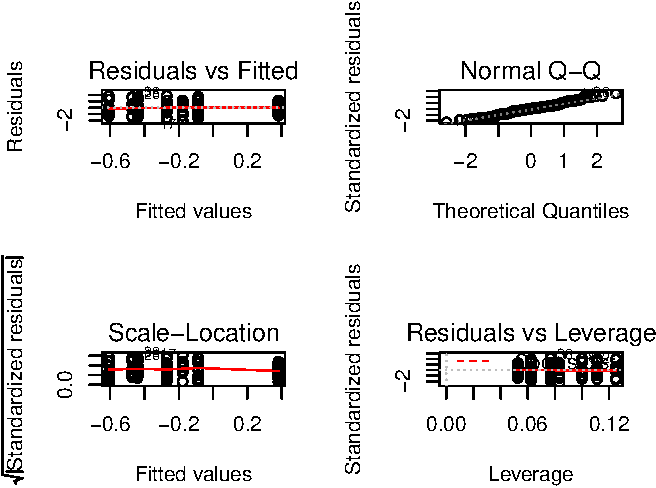
\includegraphics{04_BasicAnalyses_files/figure-beamer/unnamed-chunk-17-1.pdf}

\end{frame}

\begin{frame}[fragile]{Checking Assumptions}

They don't fit great on the slides but trust me that normality looks
good. The assumption of homogeneity of variance looks good as well.

But, if you wanted to test it, you could.

\begin{Shaded}
\begin{Highlighting}[]
\KeywordTok{library}\NormalTok{(car)}
\KeywordTok{leveneTest}\NormalTok{(fit2)}
\end{Highlighting}
\end{Shaded}

\begin{verbatim}
Levene's Test for Homogeneity of Variance (center = median)
      Df F value Pr(>F)
group  7  1.7072 0.1169
      92               
\end{verbatim}

Large p-value here is a good thing: \texttt{emo::ji("smile")}
\footnote{This shows a smiley in `R`, just not on these slides---from the `emo` package on GitHub.}

\end{frame}

\section{Linear Regression}\label{linear-regression}

\begin{frame}{Linear Regression}

\large
Once again, linear regression is essentially the more flexible twin of
ANOVA and
t-tests.\footnote{It mainly only differs from ANOVA in the way it takes a dummy code rather than an effect code of the categorical variables.}

It can:

\begin{enumerate}
\def\labelenumi{\arabic{enumi}.}
\tightlist
\item
  Handle continuous and categorical predictors (i.e., independent
  variables)
\item
  Less stringent assumption of equality of variances
\item
  Is what many other methods are built on (Chapter 5 and 6 will talk
  about some of these)
\end{enumerate}

\end{frame}

\begin{frame}[fragile]{Linear Regression}

We will use \texttt{lm()} (Linear Model) to fit these models.

\small

\begin{Shaded}
\begin{Highlighting}[]
\NormalTok{fit5 =}\StringTok{ }\KeywordTok{lm}\NormalTok{(B }\OperatorTok{~}\StringTok{ }\NormalTok{A, }\DataTypeTok{data =}\NormalTok{ df)}
\KeywordTok{summary}\NormalTok{(fit5)}
\end{Highlighting}
\end{Shaded}

\begin{verbatim}

Call:
lm(formula = B ~ A, data = df)

Residuals:
    Min      1Q  Median      3Q     Max 
-2.2052 -0.6925 -0.1018  0.6285  2.9226 

Coefficients:
            Estimate Std. Error t value Pr(>|t|)
(Intercept)  0.03416    0.14493   0.236    0.814
A1          -0.13420    0.19722  -0.680    0.498

Residual standard error: 0.9829 on 98 degrees of freedom
Multiple R-squared:  0.004703,  Adjusted R-squared:  -0.005453 
F-statistic: 0.4631 on 1 and 98 DF,  p-value: 0.4978
\end{verbatim}

\end{frame}

\begin{frame}[fragile]{Linear Regression}

We can add an interaction with the \texttt{*}. \small

\begin{Shaded}
\begin{Highlighting}[]
\NormalTok{fit6 =}\StringTok{ }\KeywordTok{lm}\NormalTok{(B }\OperatorTok{~}\StringTok{ }\NormalTok{A}\OperatorTok{*}\NormalTok{D, }\DataTypeTok{data =}\NormalTok{ df)}
\KeywordTok{summary}\NormalTok{(fit6)}
\end{Highlighting}
\end{Shaded}

\begin{verbatim}

Call:
lm(formula = B ~ A * D, data = df)

Residuals:
     Min       1Q   Median       3Q      Max 
-1.73077 -0.69977  0.02393  0.55829  2.98275 

Coefficients:
            Estimate Std. Error t value Pr(>|t|)   
(Intercept)  0.19623    0.23306   0.842  0.40198   
A1          -0.99870    0.34809  -2.869  0.00511 **
D2          -0.06529    0.40367  -0.162  0.87187   
D3          -0.20149    0.32960  -0.611  0.54250   
D4          -0.61821    0.44627  -1.385  0.16932   
A1:D2        1.52193    0.55570   2.739  0.00741 **
A1:D3        1.03230    0.48740   2.118  0.03687 * 
A1:D4        1.26047    0.56598   2.227  0.02838 * 
---
Signif. codes:  0 '***' 0.001 '**' 0.01 '*' 0.05 '.' 0.1 ' ' 1

Residual standard error: 0.9322 on 92 degrees of freedom
Multiple R-squared:  0.1595,    Adjusted R-squared:  0.09558 
F-statistic: 2.495 on 7 and 92 DF,  p-value: 0.0216
\end{verbatim}

\end{frame}

\begin{frame}[fragile]{Other Specifications}

We can also make adjustments to the variables within the model.

First, we can transform the variables (e.g., log transformation).

\begin{Shaded}
\begin{Highlighting}[]
\NormalTok{fit7 =}\StringTok{ }\KeywordTok{lm}\NormalTok{(}\KeywordTok{log}\NormalTok{(B) }\OperatorTok{~}\StringTok{ }\NormalTok{A}\OperatorTok{*}\NormalTok{D, }\DataTypeTok{data =}\NormalTok{ df)}
\KeywordTok{summary}\NormalTok{(fit7)}
\end{Highlighting}
\end{Shaded}

We can change the reference level of a variable, too.

\begin{Shaded}
\begin{Highlighting}[]
\NormalTok{fit8 =}\StringTok{ }\KeywordTok{lm}\NormalTok{(B }\OperatorTok{~}\StringTok{ }\KeywordTok{relevel}\NormalTok{(D,}\DataTypeTok{ref =} \StringTok{"4"}\NormalTok{), }\DataTypeTok{data =}\NormalTok{ df)}
\KeywordTok{summary}\NormalTok{(fit8)}
\end{Highlighting}
\end{Shaded}

\end{frame}

\begin{frame}[fragile]{Checking Assumptions}

Assumption checking is similar to that of the linear model.

\begin{Shaded}
\begin{Highlighting}[]
\KeywordTok{par}\NormalTok{(}\DataTypeTok{mfrow =} \KeywordTok{c}\NormalTok{(}\DecValTok{2}\NormalTok{,}\DecValTok{2}\NormalTok{))}
\KeywordTok{plot}\NormalTok{(fit5)}
\end{Highlighting}
\end{Shaded}

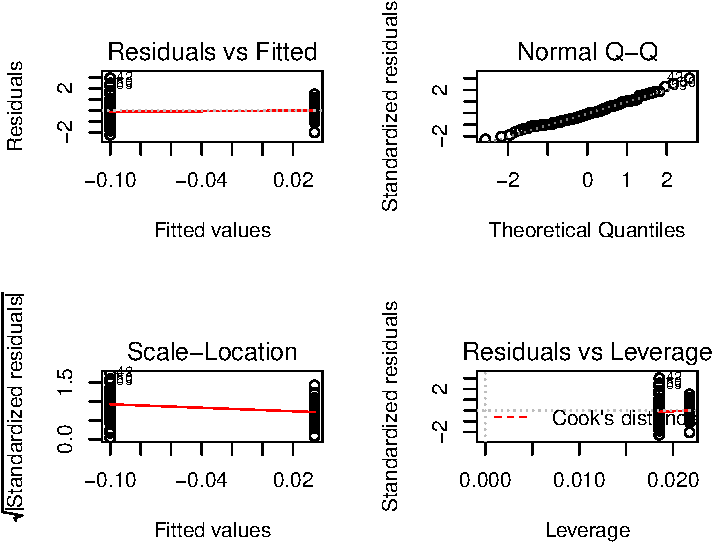
\includegraphics{04_BasicAnalyses_files/figure-beamer/unnamed-chunk-23-1.pdf}

\end{frame}

\section{Reporting Results}\label{reporting-results}

\begin{frame}[fragile]{Making This into a Table}

\Large
Often we want to present this information in a table. This can be done
is several ways:

\begin{enumerate}
\def\labelenumi{\arabic{enumi}.}
\tightlist
\item
  Pulling information out of the model objects directly
\item
  Using a package like \texttt{stargazer} to do that work for you
\item
  Manually by hand
\end{enumerate}

We can certainly do number 3 but why? So we'll look at both 1 and 2.

\end{frame}

\begin{frame}{Pull information out of the model objects}

The model objects contain loads of information that we can pull out:

\begin{enumerate}
\def\labelenumi{\arabic{enumi}.}
\tightlist
\item
  Coefficients
\item
  Standard Errors and P-values
\item
  Confidence Intervals
\item
  Fit Statistics
\item
  Predicted Values
\item
  and more! \footnote<.->{For a low cost of \$49.99! Kidding\ldots{}}
\end{enumerate}

\end{frame}

\begin{frame}[fragile]{Pull information out of the model objects}

To see what the model object holds: \small

\begin{Shaded}
\begin{Highlighting}[]
\KeywordTok{names}\NormalTok{(fit5)}
\end{Highlighting}
\end{Shaded}

\begin{verbatim}
 [1] "coefficients"  "residuals"     "effects"       "rank"         
 [5] "fitted.values" "assign"        "qr"            "df.residual"  
 [9] "contrasts"     "xlevels"       "call"          "terms"        
[13] "model"        
\end{verbatim}

\begin{Shaded}
\begin{Highlighting}[]
\KeywordTok{names}\NormalTok{(}\KeywordTok{summary}\NormalTok{(fit5))}
\end{Highlighting}
\end{Shaded}

\begin{verbatim}
 [1] "call"          "terms"         "residuals"     "coefficients" 
 [5] "aliased"       "sigma"         "df"            "r.squared"    
 [9] "adj.r.squared" "fstatistic"    "cov.unscaled" 
\end{verbatim}

\end{frame}

\begin{frame}[fragile]{Pull information out of the model objects}

\center
Using that information we can grab:

\begin{Shaded}
\begin{Highlighting}[]
\KeywordTok{summary}\NormalTok{(fit5)}\OperatorTok{$}\NormalTok{coefficients}
\end{Highlighting}
\end{Shaded}

\begin{verbatim}
              Estimate Std. Error    t value  Pr(>|t|)
(Intercept)  0.0341622   0.144925  0.2357233 0.8141393
A1          -0.1342035   0.197218 -0.6804832 0.4978031
\end{verbatim}

or

\begin{Shaded}
\begin{Highlighting}[]
\KeywordTok{summary}\NormalTok{(fit5)}\OperatorTok{$}\NormalTok{fstatistic}
\end{Highlighting}
\end{Shaded}

\begin{verbatim}
     value      numdf      dendf 
 0.4630573  1.0000000 98.0000000 
\end{verbatim}

\end{frame}

\begin{frame}[fragile]{Pull information out of the model objects}

Put it in a table:

\begin{Shaded}
\begin{Highlighting}[]
\KeywordTok{rbind}\NormalTok{(}\KeywordTok{data.frame}\NormalTok{(}\KeywordTok{summary}\NormalTok{(fit5)}\OperatorTok{$}\NormalTok{coefficients, }\StringTok{"Type"}\NormalTok{=}\StringTok{"Simple Regression"}\NormalTok{),}
      \KeywordTok{data.frame}\NormalTok{(}\KeywordTok{summary}\NormalTok{(fit6)}\OperatorTok{$}\NormalTok{coefficients, }\StringTok{"Type"}\NormalTok{=}\StringTok{"Interaction"}\NormalTok{))}
\end{Highlighting}
\end{Shaded}

\begin{verbatim}
                Estimate Std..Error    t.value    Pr...t..
(Intercept)   0.03416220  0.1449250  0.2357233 0.814139298
A1           -0.13420350  0.1972180 -0.6804832 0.497803125
(Intercept)1  0.19623455  0.2330595  0.8419935 0.401975067
A11          -0.99869651  0.3480920 -2.8690588 0.005106257
D2           -0.06528975  0.4036708 -0.1617401 0.871865234
D3           -0.20148573  0.3295959 -0.6113115 0.542500969
D4           -0.61820637  0.4462749 -1.3852591 0.169322861
A1:D2         1.52192513  0.5557046  2.7387304 0.007406153
A1:D3         1.03230395  0.4874023  2.1179709 0.036873921
A1:D4         1.26047333  0.5659765  2.2270773 0.028381762
                          Type
(Intercept)  Simple Regression
A1           Simple Regression
(Intercept)1       Interaction
A11                Interaction
D2                 Interaction
D3                 Interaction
D4                 Interaction
A1:D2              Interaction
A1:D3              Interaction
A1:D4              Interaction
\end{verbatim}

\end{frame}

\begin{frame}[fragile]{Pull information out of the model objects}

\Large
On the previous slide we:

\begin{enumerate}
\def\labelenumi{\arabic{enumi}.}
\tightlist
\item
  Created two \texttt{data.frame} with the coefficients and a variable
  called \texttt{"Type"}
\item
  Glued them together by row with \texttt{rbind()}
\end{enumerate}

This is a simple way of putting a table together that you can later
export.

\end{frame}

\begin{frame}[fragile]{Use a package like \texttt{stargazer} to do that
work for you}

A simpler but less flexible way is using a package like
\texttt{stargazer}. \tiny

\begin{Shaded}
\begin{Highlighting}[]
\KeywordTok{library}\NormalTok{(stargazer)}
\KeywordTok{stargazer}\NormalTok{(fit5, fit6, }\DataTypeTok{type =} \StringTok{"text"}\NormalTok{)}
\end{Highlighting}
\end{Shaded}

\begin{verbatim}

===========================================================
                              Dependent variable:          
                    ---------------------------------------
                                       B                   
                           (1)                 (2)         
-----------------------------------------------------------
A1                        -0.134            -0.999***      
                         (0.197)             (0.348)       
                                                           
D2                                            -0.065       
                                             (0.404)       
                                                           
D3                                            -0.201       
                                             (0.330)       
                                                           
D4                                            -0.618       
                                             (0.446)       
                                                           
A1:D2                                        1.522***      
                                             (0.556)       
                                                           
A1:D3                                        1.032**       
                                             (0.487)       
                                                           
A1:D4                                        1.260**       
                                             (0.566)       
                                                           
Constant                  0.034               0.196        
                         (0.145)             (0.233)       
                                                           
-----------------------------------------------------------
Observations               100                 100         
R2                        0.005               0.160        
Adjusted R2               -0.005              0.096        
Residual Std. Error  0.983 (df = 98)     0.932 (df = 92)   
F Statistic         0.463 (df = 1; 98) 2.495** (df = 7; 92)
===========================================================
Note:                           *p<0.1; **p<0.05; ***p<0.01
\end{verbatim}

\end{frame}

\begin{frame}[fragile]{Use a package like \texttt{stargazer} to do that
work for you}

This particular package can take several model objects and produce a
nice table. It is hard to see but it includes the number of
observations, fit statistics, the coefficients, and f-statistics.

Other packages exist that do similar things (e.g., \texttt{texreg}).

\begin{Shaded}
\begin{Highlighting}[]
\KeywordTok{library}\NormalTok{(texreg)}
\KeywordTok{screenreg}\NormalTok{(}\KeywordTok{list}\NormalTok{(fit5, fit6))}
\end{Highlighting}
\end{Shaded}

\end{frame}

\section{Conclusions}\label{conclusions}

\begin{frame}{Conclusion}

\Large

\begin{enumerate}
\item Performing linear models is straightforward in `R`
\item With a few lines of code, we can fit a model and check model assumptions
\item We can easily turn our model information into an informative table
\end{enumerate}

\end{frame}

\begin{frame}

\centerline{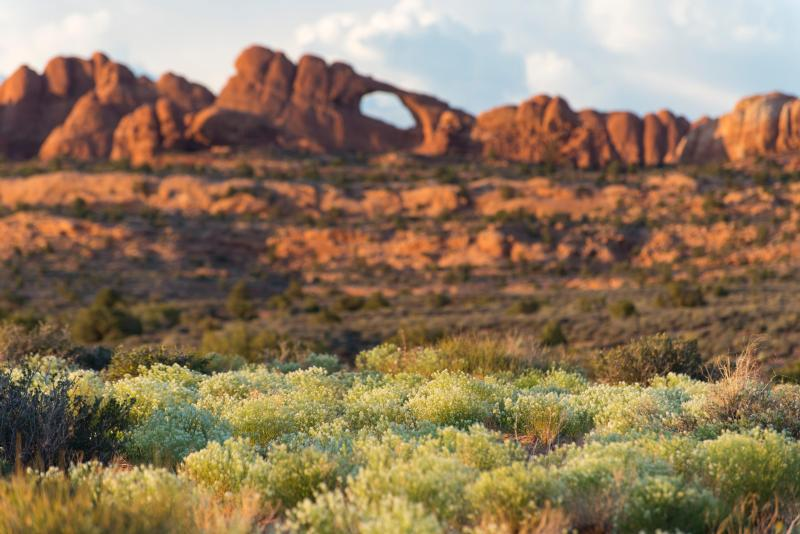
\includegraphics[height=7in]{Figures/grass_landscape_arch.jpg}}

\end{frame}
